\documentclass[12pt,a4paper,oneside,brazil]{abntex2}

% Pacotes que serão utilizados%
\usepackage{lmodern}
\usepackage[utf8]{inputenc}
\usepackage[brazil]{babel}
\usepackage[T1]{fontenc}
\usepackage{indentfirst}
\usepackage{graphicx}
\usepackage{microtype}
\usepackage{wrapfig}
\usepackage{amsmath}
\usepackage[backend=biber, style=abnt]{biblatex}
\addbibresource{Referencias.bib}

% Informações do documento %
\title{Notas Micro I}
\author{Thiago Oliveira Coelho}
\date{\today}



\begin{document}
\pagestyle{plain}
\pagenumbering{arabic}
\maketitle
\begin{center}
Resumo baseado em \cite{mas}, \cite{nicholson}, \cite{varian} e \cite{pindyck}
\end{center}
\tableofcontents

\chapter{1ª Unidade}

\section{Escolha do consumidor}

Sendo $A \succ B$ lido como A preferível a B, temos os axiomas da escolha racional:

\begin{enumerate}
\item Complitude: Se $A \succ B$ então $B \nsucc A$;
\item Transitividade: Se $A \succ B$ e $B \succ C$ então $A \succ C$;
\end{enumerate} 

Cada cesta de bens terá um valor em utilidade subjetiva para cada consumidor.
Pela dificuldade de lidar com grandezas deste tipo, nos preocuparemos não com o
valor nominal da utilidade, mas sim com a ordem de cestas que produzem mais ou 
menos utilidade para o consumidor. Esta utilidade se dá da seguinte forma:

\begin{equation} \label{utilidade}
Utilidade = U(x_1, x_2, x_3, .... ,x_n)
\end{equation}

Sendo x Os vários bens que podem estar inclusos nesta cesta. Para fins de
simplificação, em geral lidaremos com cestas de dois bens. A palavra "bens" é 
usada para melhorar a didática, mas podemos utilizar a análise microeconômica 
para obter o resultado ótimo em todo tipo de situação:

\[ Utilidade = U(H_t, H_l) \]

Sendo $H_t$ horas trabalhadas e $H_l$ horas de lazer. Ao analisarmos dois bens,
uma das ferramentas mais poderosas que podemos utilizar é a das curvas de 
indiferença, que nos diz todas as combinações de bens que retornam certo nível 
constante de utilidade ao consumidor.

\begin{figure}[ht]
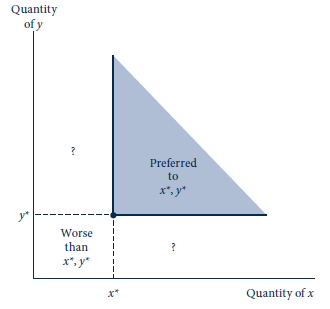
\includegraphics[scale=0.70]{Curva de indiferenca.png}
\centering
\caption{Fonte: \cite[p. 93]{nicholson}}
\end{figure}

A área azul representa todas as cestas estritamente preferidos a cesta 
analisada, já as cestas presente nas áreas (?) ficam indefinidas: como possuem 
mais de um bem e menos de outro, podem ser melhores ou piores. Começamos a 
introduzir a curva de indiferença calculando a inclinação delas:

\printbibliography

\end{document}
